\documentclass[12pt, a4paper]{extreport}

% --- CÁC GÓI CẦN THIẾT ---
\usepackage[utf8]{inputenc}
\usepackage[T5]{fontenc} 
\usepackage[vietnamese]{babel}
\usepackage{geometry}
\usepackage{times} 
\usepackage{graphicx} 
\usepackage{titlesec}
\usepackage{tocloft}
\usepackage{tikz}
\usepackage{setspace}
\usepackage{eso-pic} 
\usepackage{float} 
\usepackage{ragged2e}
\usepackage{array}
\usepackage{longtable}
\usepackage{subcaption}
\usepackage{tikz}
\usepackage{hyperref}
\usetikzlibrary{positioning, arrows.meta, shapes.multipart}

% Thiết lập lề cho tài liệu
\geometry{a4paper, top=2.5cm, bottom=2.5cm, left=2.5cm, right=2.5cm}

% --- ĐỊNH DẠNG ĐÁNH SỐ ĐỀ MỤC ---

\renewcommand{\thechapter}{\Roman{chapter}}
\renewcommand{\thesection}{\arabic{section}}
\renewcommand{\thesubsection}{\thesection.\arabic{subsection}}
\renewcommand{\thesubsubsection}{\thesubsection.\arabic{subsubsection}}
\renewcommand{\theparagraph}{\alph{paragraph})}

% --- ĐỊNH DẠNG ĐÁNH SỐ HÌNH ẢNH/BẢNG BIỂU SỐ Ả RẬP ---
\renewcommand{\thefigure}{\arabic{chapter}.\arabic{figure}}
\renewcommand{\thetable}{\arabic{chapter}.\arabic{table}}

% --- ĐỊNH DẠNG TIÊU ĐỀ (titlesec) ---

\titleformat{\chapter}[block]
  {\normalfont\Large\bfseries\centering}
  {CHƯƠNG \thechapter. }
  {0pt}
  {\MakeUppercase}
\titlespacing*{\chapter}{0pt}{-20pt}{20pt}

\titleformat{\section}
  {\normalfont\large\bfseries}
  {\thesection. }
  {0.3em}
  {}

\titleformat{\subsection}
  {\normalfont\normalsize\bfseries}
  {\thesubsection. }
  {0.3em}
  {}

\titleformat{\subsubsection}
  {\normalfont\normalsize\bfseries}
  {\thesubsubsection. }
  {0.3em}
  {}

\titleformat{\paragraph}[runin]
  {\normalfont\normalsize\bfseries}
  {\theparagraph \space}
  {0pt}
  {}
\titlespacing*{\paragraph}{0pt}{1ex}{1em}

% --- ĐỊNH DẠNG MỤC LỤC (tocloft) ---

\renewcommand{\cftchappresnum}{CHƯƠNG }
\renewcommand{\cftchapaftersnum}{.}
\setlength{\cftchapnumwidth}{7.5em} 

\setlength{\cftsecindent}{0pt}
\setlength{\cftsecnumwidth}{2em}
\setlength{\cftsubsecindent}{1.5em}
\setlength{\cftsubsecnumwidth}{2.5em}
\setlength{\cftsubsubsecindent}{3.5em}
\setlength{\cftsubsubsecnumwidth}{3em}

\setcounter{secnumdepth}{4} % Đánh số đến tận mục paragraph (a, b, c)
\setcounter{tocdepth}{3}    % Hiển thị đến mục 1.1.1 trong mục lục
\usepackage{lmodern}

\onehalfspacing 

% --- BẮT ĐẦU TÀI LIỆU ---
\begin{document}
\setlength{\parindent}{0pt}
\setlength{\parskip}{5pt}

% --- TRANG BÌA ---
\begin{titlepage}

\thispagestyle{empty}
\centering

% ===== VIỀN HOA VĂN (ẢNH) =====
\AddToShipoutPictureBG{
  \begin{tikzpicture}[remember picture,overlay]
    \node [
      xshift=0cm, % đẩy sang phải (chừa gáy)
      yshift=0cm
    ]
    at (current page.center) {
      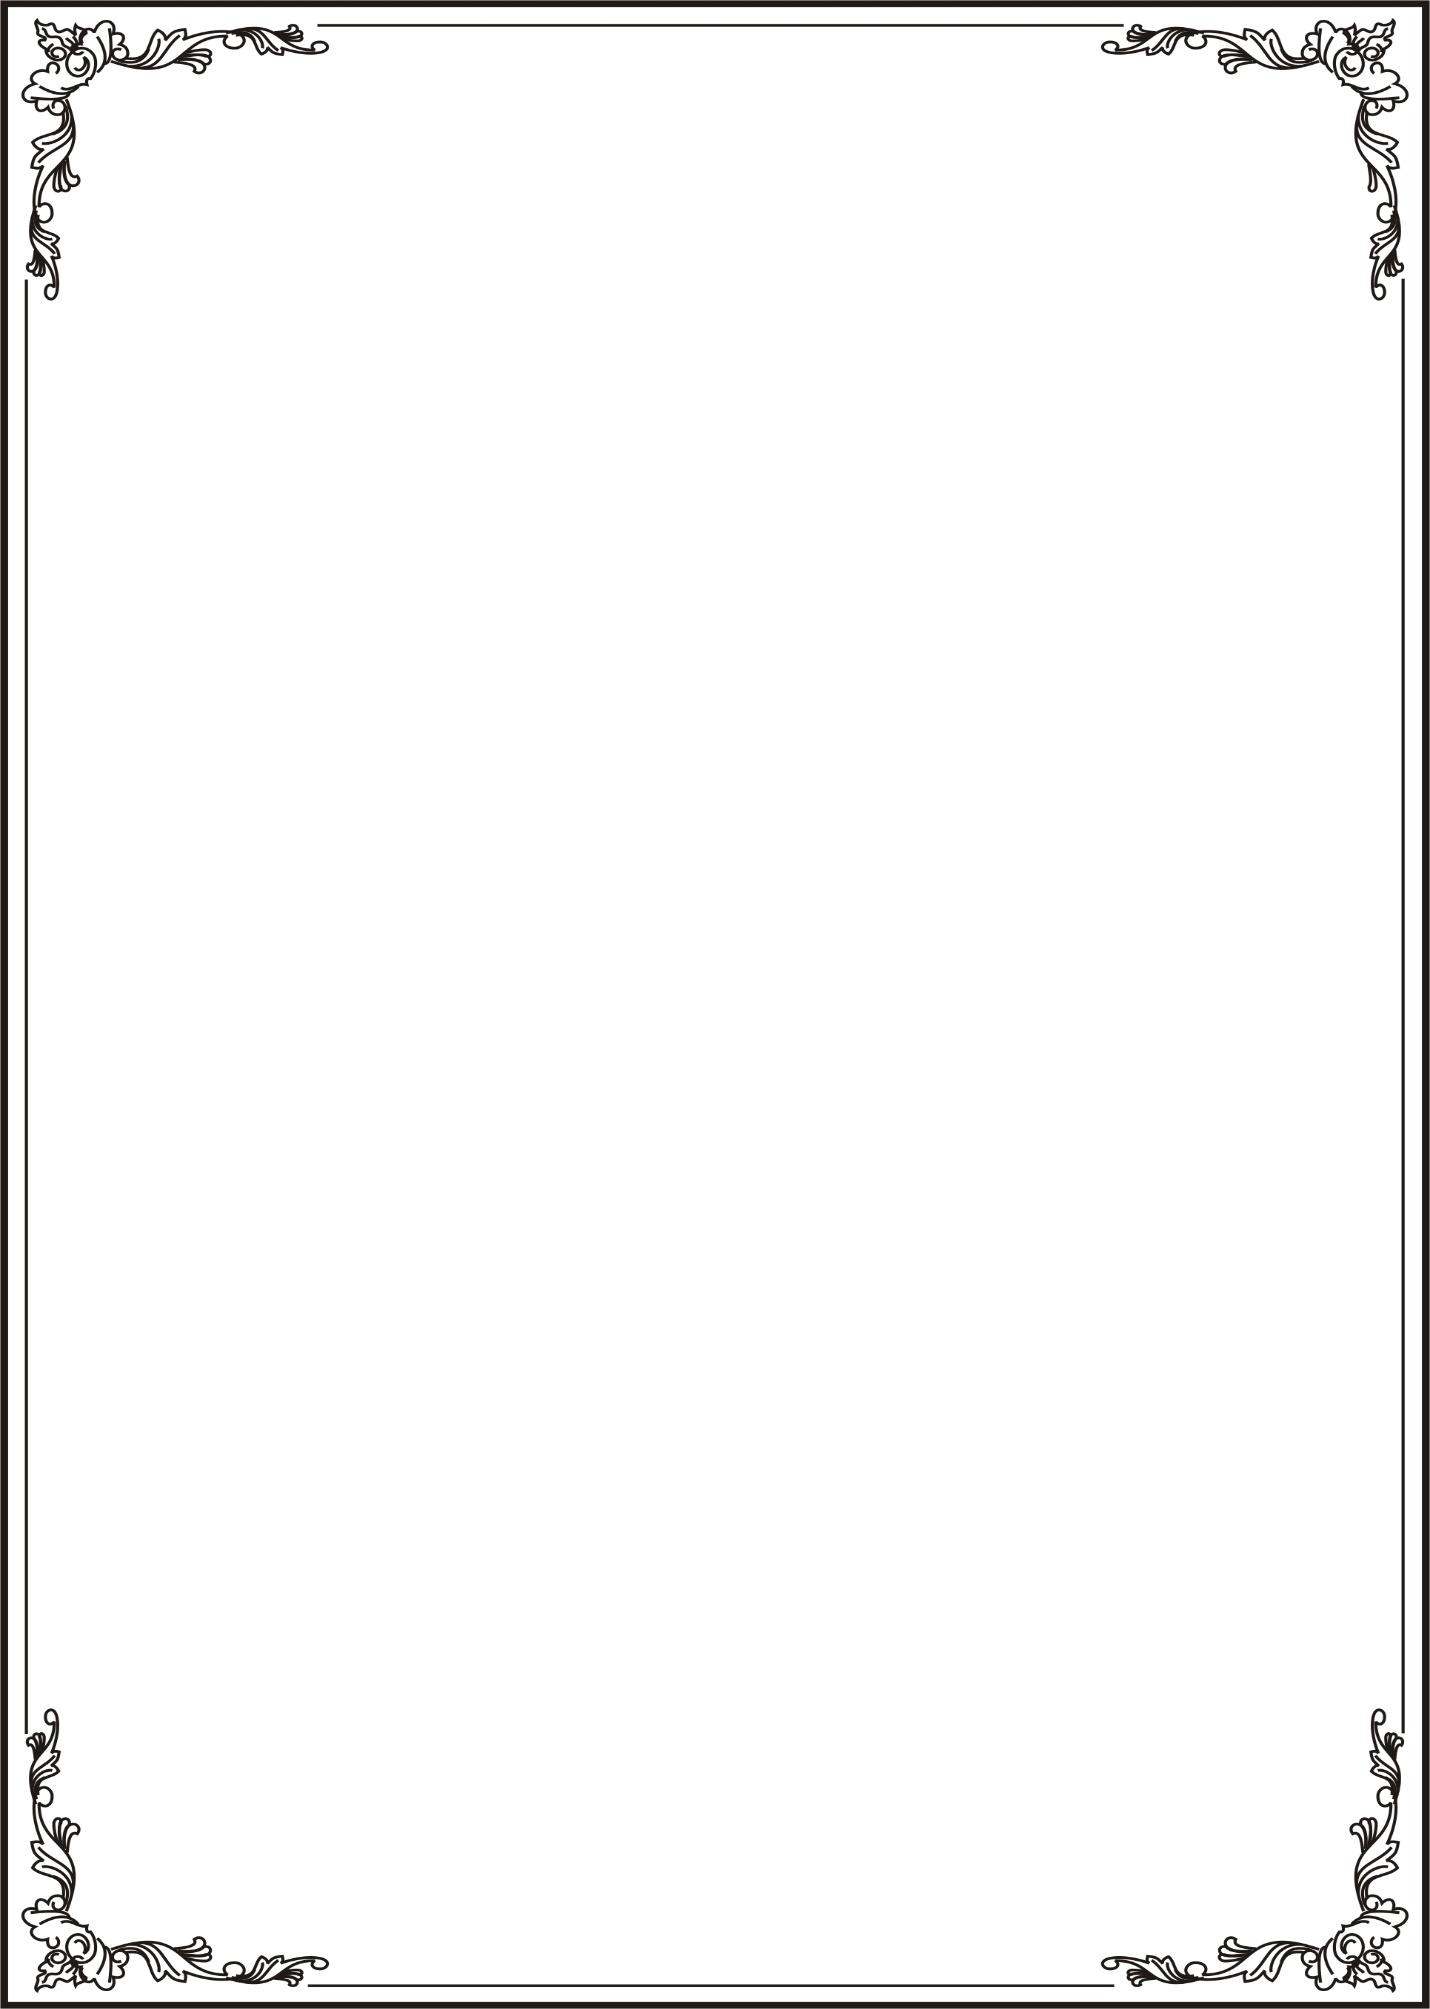
\includegraphics[
        width=0.85\paperwidth,
        height=0.9\paperheight
      ]{border.jpeg}
    };
  \end{tikzpicture}
}


\begin{center}
  \textbf{\Large TRƯỜNG ĐẠI HỌC THỦY LỢI}\\[0.3cm]
  \textbf{\large KHOA CÔNG NGHỆ THÔNG TIN}

  \vspace{0.8cm}

  
\includegraphics[width=5cm]{logo.jpeg}

  \vspace{0.8cm}

  \textbf{\Large BÀI TẬP LỚN MÔN \\ KHAI PHÁ DỮ LIỆU}\\[0.3cm]

  \vspace{0.4cm}

  \textbf{\Large ĐỀ TÀI: Phát hiện hành vi bất thường theo ngữ cảnh trên camera giám sát dựa trên phân cụm hành vi-không gian–thời gian và khai phá luật kết hợp}
  
  \vspace{0.8cm}\textbf{\large Giảng viên phụ trách môn học: Th.S Trần Mạnh Tuấn}

  \vspace{0.8cm}\textbf{\large Nhóm thực hiện: } \large Nhóm 14
  
  \vspace{0.4cm}\textbf{\large Thành viên nhóm: }

  \vspace{0.4cm}
  \begin{tabular}{p{5cm} p{3cm}}

  \end{tabular}
  
\end{center}

\vspace{1cm}

\vfill

\begin{center}
  \textit{Hà Nội, 15 tháng 5 năm 2026}
\end{center}
\end{titlepage}
\ClearShipoutPictureBG


% --- MỤC LỤC ---
\tableofcontents
\newpage

% --- DANH MỤC VIẾT TẮT ---
% \input{sections/abbreviations.tex}
\newpage

% --- NỘI DUNG BÁO CÁO ---

% Mô tả đề tài
\chapter{Mô tả đề tài}

\section{Tên đề tài}

\textbf{Phát hiện hành vi bất thường theo ngữ cảnh trên camera giám sát dựa trên phân cụm hành vi-không gian--thời gian và khai phá luật kết hợp}

\section{Mục tiêu}

\subsection{Mục tiêu tổng quát}

Đề tài hướng tới xây dựng một phương pháp hỗ trợ hệ thống camera giám sát có khả năng tự động phân tích video và cảnh báo các hành vi bất thường dựa trên cả đặc trưng chuyển động lẫn ngữ cảnh xuất hiện của hành vi.

\subsection{Mục tiêu cụ thể}

\begin{itemize}
    \item Trích xuất các đặc trưng hành vi-không gian--thời gian từ video giám sát.
    \item Phân cụm các hành vi tương tự để hình thành các mẫu hành vi bình thường thường gặp trong cảnh.
    \item Khai phá các luật kết hợp giữa hành vi và ngữ cảnh như vị trí, thời gian, loại đối tượng hoặc hướng di chuyển.
    \item Phát hiện các hành vi lệch khỏi mẫu bình thường hoặc xuất hiện trong bối cảnh không phù hợp.
    \item Hỗ trợ đưa ra cảnh báo có khả năng giải thích cho người vận hành.
\end{itemize}

\section{Phương pháp}

Phương pháp đề xuất kết hợp ba thành phần chính: trích xuất đặc trưng hành vi-không gian--thời gian, phân cụm hành vi và khai phá luật kết hợp ngữ cảnh.

\subsection{Trích xuất đặc trưng hành vi-không gian--thời gian}

Từ video camera giám sát, hệ thống thu thập các thông tin như vị trí, tốc độ, hướng di chuyển, thời gian xuất hiện, vùng đi qua, thời gian dừng và các đặc điểm quỹ đạo khác. Những thông tin này được kết hợp để tạo thành biểu diễn đặc trưng cho từng hành vi.

\subsection{Phân cụm hành vi}

Các đặc trưng sau khi trích xuất được đưa vào thuật toán phân cụm nhằm tìm ra các nhóm hành vi bình thường thường lặp lại trong cảnh, chẳng hạn như đi thẳng, rẽ, dừng, đứng lâu hoặc di chuyển theo các hướng quen thuộc.

\subsection{Khai phá luật kết hợp ngữ cảnh}

Từ kết quả phân cụm và thông tin ngữ cảnh, hệ thống xây dựng các giao dịch hành vi và khai phá các luật phổ biến, ví dụ:

\begin{itemize}
    \item người đi bộ thường xuất hiện trên vỉa hè;
    \item xe thường di chuyển trong làn xe;
    \item một số hành vi chỉ thường xảy ra tại các vùng hoặc thời điểm nhất định.
\end{itemize}

Một hành vi được xem là bất thường khi nó lệch xa các cụm hành vi bình thường hoặc vi phạm các luật ngữ cảnh đã khai phá.

\section{Cách triển khai}

\subsection{Giai đoạn 1: Chuẩn bị dữ liệu}

Lựa chọn các bộ dữ liệu video giám sát công khai phù hợp như UCSD Pedestrian, CUHK Avenue, ShanghaiTech Campus, Street Scene hoặc NWPU Campus.

\subsection{Giai đoạn 2: Tiền xử lý video}

\begin{itemize}
    \item Chuẩn hóa video.
    \item Phát hiện vùng chuyển động.
    \item Theo dõi đối tượng.
    \item Chia cảnh thành các vùng không gian.
\end{itemize}

\subsection{Giai đoạn 3: Trích xuất đặc trưng}

Tạo tập dữ liệu có cấu trúc gồm các đặc trưng về chuyển động, vị trí, thời gian, quỹ đạo và vùng xuất hiện.

\subsection{Giai đoạn 4: Phân cụm hành vi}

Áp dụng thuật toán phân cụm để xác định các mẫu hành vi bình thường trong từng cảnh.

\subsection{Giai đoạn 5: Khai phá luật kết hợp}

Chuyển các hành vi thành giao dịch ngữ cảnh và sinh ra các luật hành vi thường gặp.

\subsection{Giai đoạn 6: Phát hiện bất thường}

Kết hợp độ lệch khỏi cụm hành vi và mức độ vi phạm luật ngữ cảnh để tính điểm bất thường và sinh cảnh báo.

\subsection{Giai đoạn 7: Đánh giá}

Đánh giá hiệu quả của phương pháp bằng các chỉ số như Precision, Recall, F1-score, ROC-AUC, tỷ lệ cảnh báo giả và thời gian xử lý.

\section{Kết quả kỳ vọng}

\begin{itemize}
    \item Xây dựng được mô hình phát hiện hành vi bất thường theo ngữ cảnh trên video giám sát.
    \item Phát hiện được cả hành vi lạ và hành vi quen thuộc nhưng xảy ra sai bối cảnh.
    \item Giảm cảnh báo giả so với phương pháp chỉ xét chuyển động.
    \item Tạo ra được các cảnh báo có khả năng giải thích, hỗ trợ người vận hành giám sát hiệu quả hơn.
\end{itemize}


% Lời nói đầu
% \input{sections/preface.tex}
% % Chương 1
% \input{sections/chapter1.tex}

% % Chương 2
% \input{sections/chapter2.tex}

% % Chương 3
% \input{sections/chapter3.tex}

% % Chương 4
% \input{sections/chapter4.tex}

% % Kết luận
% \chapter{Ket luan va huong phat trien}

\section{Muc da hoan thanh}

Pipeline hien tai da co cac thanh phan chinh theo PRD: tien xu ly video, chia grid/cube, feature motion/brightness, phan cum MiniBatchKMeans theo cell, token/rule, scoring, smoothing, heatmap va casebook giai thich. SPEC 10 dong goi cac artifact nay thanh section LaTeX, bang tom tat, hinh minh hoa va manifest de tai lap.

\section{Han che}

\begin{itemize}
  \item Grid hien tai chua phai zone ngu nghia do nguoi dung ve.
  \item Rule support co the thap va chi nen doc nhu tin hieu giai thich phu.
  \item Smoke artifact khong thay the cho danh gia benchmark day du.
  \item Manual review trong casebook van de \texttt{TBD}, nen khong gan nhan true positive/false positive trong bao cao chinh.
\end{itemize}


\section{Huong phat trien}

Huong tiep theo la review thu cong mot tap case tieu bieu, bo sung zone ngu nghia, thu object detector nhe khi can phan biet nguoi/xe, va mo rong bao cao bang phu luc tai lap pipeline khi artifact production day du hon.


\end{document}
